\section{Architecture and implementation}\label{sec:architecture}

\subsection{YETI standalone application}
YETI is an automated random testing tool for Java. 
A YETI testing session consists in a sequence of calls made to methods at
random using arguments generated at random. 
The oracle for the tests are either contracts --�when available -- or runtime 
exceptions/failures.

When a failure is detected the logs of the testing session are minimised to 
produce test cases that reproduce the failure. Such unit tests can then be stored and 
be executed later by a unit test framework.

YETI is usually launched on the command-line. A typical call to YETI is:
{\small
\begin{verbatim}
java yeti.Yeti -Java -yetiPath=. 
          -time=10mn -randomPlus
          -testModules=String:StringBuilder 
\end{verbatim}
}

The options used on this command-line have the following meaning: \texttt{-Java} 
indicates that the tested program is in Java, \texttt{-yetiPath=.} indicate that 
classes in the current directory (and its subdirectories) will be preloaded, 
\texttt{-time=10mn} indicates that the testing session will last 10 minutes, 
\texttt{-randomPlus} indicates that the strategy random+~\cite{CMOP:08:FFMTRTUR} will be used, and 
\texttt{-testModules=String:StringBuilder} indicates that 
both \texttt{String} and \texttt{StringBuilder} will be tested.

While testing, traces of faults found are output to the terminal. For example:

{\small
\begin{verbatim}
Exception 5
java.lang.NullPointerException
 at java.lang.String.replace(String.java:2207)
\end{verbatim}
}

At the end of the testing sessions, YETI outputs generated test cases reproducing 
the faults found during the testing session as well.

Note that it is possible to avoid the overhead of keeping the 
traces in the system (and calculating the minimal test cases) by specifying 
\texttt{-nologs} to throw away all logs except exception traces, or 
\texttt{-rawlogs} to output the logs to the terminal. This comes at the cost of
not being able to generate test cases reproducing the failures, but still provides 
the exception traces. In an exploratory phase of the testing, this is generally the
way to use YETI.


\begin{figure}[h]
\begin{center}
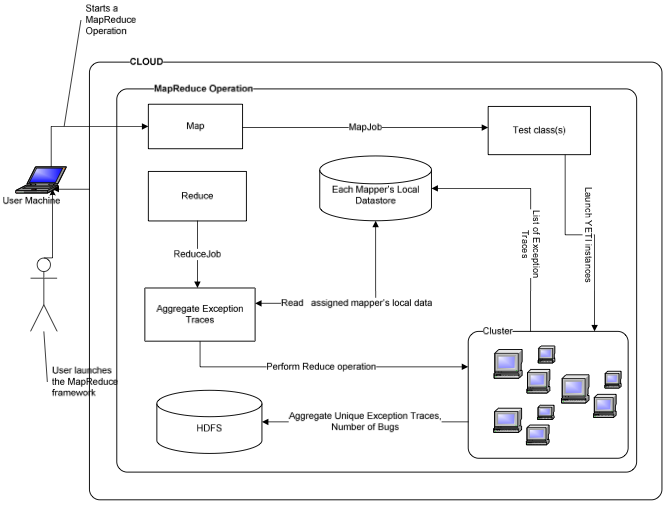
\includegraphics[width=\columnwidth]{images/YetiCloud.png}
\end{center}
\caption{YETI cloud architecture.}\label{fig:architecture}
\end{figure}


\subsection{Architecture of the cloud implementation}

As figure~\ref{fig:architecture} shows, the main architecture of YETI on the cloud 
relies on Hadoop, Apache's implementation of Google's map/reduce framework. 

The main idea is that we use a very simple approach where testing jobs 
are described by calls to YETI stored in normal text files by the user, that will each launch YETI in standalone mode. 
Commands from within each file are then mapped to different machines in the cloud. 

After setting up the map/reduce cluster. These text files and YETI (bundled as a jar file) are then uploaded to the 
distributed file system (DFS) on the map/reduce cluster master, which then launches individual testing machines 
for each text file executing the commands contained within the file in the order they appear.

At the end of the testing session, all exception traces are written back to the DFS during reduce step, which can then be downloaded to the 
user machine and made available to the software tester for evaluation.


\subsection{Evaluation}

We only ran preliminary evaluations.

We evaluated our approach using the Amazon Elastic Computing Cloud (EC2) \footnote{http://aws.amazon.com/ec2/}.
We performed 5 jobs of 20-minutes each (a total testing time of 100 minutes) in less 
than 21 minutes, outputting comparable results with YETI's standalone execution. 
Test cases all tested classes from \texttt{java.lang}.
The number of faults found in each tested class in the distributed mode were the same as those found during standalone execution of YETI. 

By using the cloud we clearly improved the performances of YETI and reduce the testing time by 
employing more machines and distributing the jobs. 
Distributing YETI over the cloud requires uploading the files containing typical YETI calls for launching YETI in standalone mode(multiple 
YETI calls can be placed in a file resulting in the same machine testing different or the same files with different options/strategies), and 
YETI itself (bundled as a Jar along with the classes to be tested). Setting up Hadoop cluster on EC2  and uploading all the required files to the 
MapReduce Master would then need under a few minutes. However, setting up the EC2 cluster for the first time might 
take some  extra time(up to 10 minutes), but subsequent testing sessions would require under a few minutes to start, making it a suitable 
candidate for regression testing. 
The execution can be performed on a locally set up Hadoop cluster as well. While we did not run experiments with 
more open security models, YETI jobs were run on one-shot Ubuntu virtual machines. This also solves
the potential security issues for random testing.
